\section{Proposed algorithm}
\label{sec_algo}

\subsection{Learning multi-task policy from offline data with distillation}\label{sec_algo_distillation}

In Multi-task RL, \cite{rusu2015policy, teh2017distral, ghosh2017divide,czarnecki2019distilling, ActorMimicParisotto2015} demonstrate the success of distilling multiple single-task policies into a multi-task policy. Inspired by these works, we propose a distillation procedure to obtain a multi-task policy in the Multi-task Batch RL setting. In Sec. \ref{sec_algo_triplet}, we argue such distillation procedure alone is insufficient due to the constraints the batch setting imposes on the policy search procedure.

The distillation procedure has two phases.
In the first phase, we use BCQ to learn a different policy for each task, i.e. we learn $K$ different and independent policies. While we can use any Batch RL algorithm in the first phase, we use BCQ due to its simplicity.
As described in Sec. \ref{BCQ},
for each training batch, BCQ learns three functions: a state-action value function $Q$, a candidate action generator $G$ and a perturbation generator $\xi$. The output of the first phase thus consists of three sets of networks $\{Q_i\}^K_{i=1}$, $\{G_i\}^K_{i=1}$, and $\{\xi_i\}^K_{i=1}$, where $i$ indexes over the training tasks.

In the second phase, we distill each set into a network by incorporating a task inference module. The distilled function should recover different task-specific function depending on the inferred task identity. To distill the value functions $\{Q_i\}^K_{i=1}$ into a function $Q_D$, for each task $i$, we sample a context ${\bf c}_{i}$ and a pair $(s, a)$ from the batch $\mathcal{B}_i$. The task inference module $q_\phi$ takes ${\bf c}_{i}$ as input and infers a task identity ${\bf z}_i$. Given ${\bf z}_i$ as input, $Q_D$ should assign similar value to $(s, a)$ as the value function for the $i^{th}$ task $Q_i(s, a)$. The loss function with a $\beta$-weighted KL term \cite{rakelly2019efficient} is:
\begin{equation}\label{eq_loss_qi}
    \mathcal{L}_Q = \frac{1}{K} \sum_{i=1}^{K} \mathlarger{\underset{\substack{(s, a),  {\bf c}_{i} \sim  \mathcal{B}_i }}{\mathbb{E}} }\left[( Q_i(s, a) - Q_D(s, a, {\bf z}_i) )^2 + \beta\text{KL}(q_\phi({\bf c}_i) ||  \mathcal{N}(0,1))\right], \, {\bf z}_i \sim q_\phi({\bf c}_{i})
\end{equation}
We also use Eq. \ref{eq_loss_qi} to train $q_\phi$ using the reparam trick \cite{kingma2013auto}. Similarly, we distill the candidate action generators $\{G_i\}^K_{i=1}$ into $G_D$. $G_D$ takes as input state $s$, random noise $\nu$ and task identity ${\bf z}_i$. Depending on ${\bf z}_i$'s value, we train $G_D$ to regress towards the different candidate action generator:
\begin{equation}\label{eq_loss_gi}
    \mathcal{L}_G = \frac{1}{K} \sum_{i=1}^{K} \mathlarger{\underset{\substack{s, {\bf c}_{i} \sim \mathcal{B}_i \\ \nu \sim \mathcal{N}(0,1) }}{\mathbb{E}} } \left[ || G_i(s, \nu) - G_D(s, \nu, \bar{\bf z}_i) || ^ 2 \right], \quad {\bf z}_i \sim q_\phi({\bf c}_{i}).
\end{equation}

The bar on top of $\bar{\bf z}_i$ in Eq. \ref{eq_loss_gi} indicates the stop gradient operation. We thus do not use the gradient of Eq. \ref{eq_loss_gi} to train the task inference module \cite{rakelly2019efficient}. Lastly, we distill the perturbation generators $\{\xi_i\}^K_{i=1}$ into a single network $\xi_D$ (Eq. \ref{eq_loss_xi_i}).
$\xi_D$ takes as input a state $s$, a candidate action $a$, and an inferred task identity ${\bf z}_i$. We train $\xi_D$ to regress towards the output of $\xi_i$ given the same state $s$ and candidate action $a$ as input.
We obtain the candidate action $a$ by passing $s$ through the candidate action generator $G_i$.
\begin{equation}\label{eq_loss_xi_i}
    \mathcal{L}_\xi = \frac{1}{K} \sum_{i=1}^{K} \mathlarger{\underset{\substack{s, {\bf c}_{i} \sim \mathcal{B}_i \\ \nu \sim \mathcal{N}(0,1)} }{\mathbb{E}}}\left[ || \xi_i(s, a) - \xi_D(s, a, \bar{\bf z}_i) || ^ 2 \right], \quad {\bf z}_i \sim q_\phi({\bf c}_{i}), \quad a = G_i(s, \nu)
\end{equation}
Note that the gradient of $\mathcal{L}_\xi$ also updates $G_i$. The final distillation loss is given in Eq. \ref{eq_distill_loss}. We parameterize $q_\phi, Q_D, G_D, \xi_D$ with feedforward NN as detailed in Appendix \ref{sec_hp_distillation}.
\begin{equation}\label{eq_distill_loss}
    \mathcal{L}_{distill} = \mathcal{L}_Q + \mathcal{L}_G + \mathcal{L}_\xi.
\end{equation}

\subsection{Robust task inference with triplet loss design}\label{sec_algo_triplet}

% \begin{wrapfigure}{R}{0.269\textwidth}
%     \centering
%     \vspace{-0.5em}
%     \begin{subfigure}{0.15\paperwidth}
%         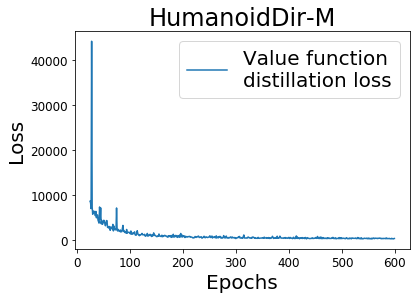
\includegraphics[width=\linewidth]{chapter_2/fig/HumanoidDir-M-neither-qloss.png}
%     \end{subfigure}

%     \begin{subfigure}{0.15\paperwidth}
%         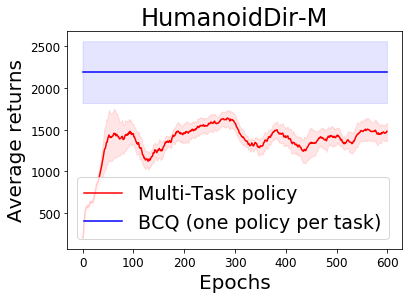
\includegraphics[width=\linewidth]{chapter_2/fig/HumanoidDir-M-neither-train-returns.png}
%     \end{subfigure}
%     \caption{{\bf Top:} Value function
%         distillation
%         loss (Eq. \ref{eq_loss_qi}) during training. {\bf Bottom:} The performance of the multi-task policy trained with Eq. \ref{eq_distill_loss} versus BCQ.}\label{fig:fail-distill}
% \end{wrapfigure}

Given the high performance of distillation in Multi-task RL \cite{rusu2015policy, teh2017distral, ghosh2017divide,czarnecki2019distilling, ActorMimicParisotto2015}, it surprisingly performs poorly in Multi-task Batch RL, even on the training tasks. This is even more surprising because we can minimize the distillation losses (Fig. \ref{fig:fail-distill} top) and the single-task BCQ policies have high performance (Fig. \ref{fig:fail-distill} bottom). If the single-task policies perform well and we can distill them into a multi-task policy, why does the multi-task policy have poor performance? We argue the task inference module has learnt to model the posterior over task identity as conditionally dependent on only the state-action pairs in the context set
, i.e. $P(Z|S, A)$,
where $S, A$ are random variables denoting states and actions, rather than the correct dependency $P(Z|S, A, R)$ where $R$ denotes the rewards.

The behavior of the trained multi-task policy supports this argument. In this experiment, each task corresponds to a running direction. To maximize returns, the policy should run with maximal velocity in the target direction. We found that the multi-task policy often runs in the wrong target direction, indicating incorrect task inference.
At the beginning of evaluation, the task identity is not provided.
% \jiachen{In evaluation, the task identity is not provided.}
The policy takes random actions, after which it uses the collected transitions to infer the task identity.
Having learnt the wrong conditional dependency, the task inference module assigns high probability mass in the posterior to region in the task embedding space whose training batches overlap with the collected transitions (Fig. \ref{fig:cheat}).

The fundamental reason behind the wrong dependency is the non-overlapping nature of the training batches.
Minimizing the distillation loss does not require the policy to learn the correct but more complex dependency.
The multi-task policy should imitate different single-task policy depending on which batch the context set was sampled from.
If the batches do not overlap in state-action visitation frequencies, the multi-task policy can simply correlate the state-action pairs in the context with which single-task policy it should imitate. In short, if minimizing the training objective on the given datasets does not require the policy to model the dependency of the task identity on the rewards in the context set, there is no guarantee the policy will model this dependency. This is not surprising given literature on the non-identifiability of causality from observations \cite{pearl_2009, Peters2017}. They also emphasize the benefit of using distribution change as training signal to learn the correct causal relationship \cite{Bengio2020A}.

Inspired by this literature, we introduce a distribution change into our dataset by approximating the reward function of each task $i$ with a learned function $\hat{R}_i$ (training illustrated in \autoref{sec_ensemble}). Given a context set ${\bf c}_j$ from task $j$, we relabel the reward of each transition in ${\bf c}_j$ using $\hat{R}_i$. Let $t$ index the transitions and ${\bf c}_{j\rightarrow{i}}$ denote the set of the relabelled transitions, we illustrate this process below :
\begin{equation}\label{eq_relabel}
    \quad {\bf c}_{j}=\left\{ \left(s_{j, t}, a_{j, t}, r_{j, t}, s_{j, t}^{\prime}\right) \right\}_t   \xrightarrow{\text{Relabelling}} {\bf c}_{j\rightarrow{i}} = \left\{ \left(s_{j, t}, a_{j, t}, \hat{R}_i(s_{j, t}, a_{j, t}), s_{j, t}^{\prime} \right) \right\}_t
\end{equation}
Given the relabelled transitions, we leverage the triplet loss from the metric learning community \cite{hermans2017defense} to enforce robust task inference, which is the most important design choice in MBML. Let $K$ be the number of training tasks, ${\bf c}_i$ be a context set for task $i$, ${\bf c}_j$ be
a context set for task $j$ ($j \neq i$)
, and ${\bf c}_{j\rightarrow{i}}$ be the relabelled set as described above, the triplet loss for task $i$ is:
\begin{equation}\label{eq_triplet_task_i}
    \mathcal{L}^i_{triplet} = \frac{1}{K-1} \sum_{j=1, j \neq i }^{K} \bigg[\explain{d \big(q_{\phi}\left({\bf c}_{j\rightarrow{i}}\big), q_{\phi}\left({\bf c}_{i}\right)\right) \quad}{Ensure ${\bf c}_{j\rightarrow{i}}$ and ${\bf c}_{i}$ infer \textit{similar} task identities \quad}
        - \explain{ \quad d\big(q_{\phi}\left({\bf c}_{j\rightarrow{i}}\right), q_{\phi}\left({\bf c}_{j}\right)\big) \quad}{Ensure ${\bf c}_{j\rightarrow{i}}$ and ${\bf c}_{j}$ infer \textit{different} task identities} + \quad m\bigg]_{+},
\end{equation}

\begin{figure}[!t]
    \begin{minipage}{0.5\textwidth}
        \begin{algorithm}[H]
            \caption{Distillation and triplet loss}\label{algo_mtbrl}
            {\bf Input}: Batches $\{\mathcal{B}_{i}\}_{i=1}^K$; BCQ-trained $\{Q_i\}^K_{i=1}$, $\{G_i\}^K_{i=1}$, and $\{\xi_i\}^K_{i=1}$; randomly initialized $Q_D$, $G_D$ and $\xi_D$ jointly parameterized by $\theta$; task inference module $q_\phi$ with randomly initialized $\phi$
            \begin{algorithmic}[1]
                \Repeat
                \State Sample context set ${\bf c}_i$ from $\mathcal{B}_{i}, \forall i$
                \State Obtain relabelled transitions ${\bf c}_{j\rightarrow i}$ according to Eq. \ref{eq_relabel} for all pair of task $i, j$
                \State Calculate $\mathcal{L}_{triplet}$ using Eq. \ref{eq_triplet_all_task}
                \State Calculate $\mathcal{L}_Q, \mathcal{L}_G, \mathcal{L}_\xi$ using Eq. \ref{eq_loss_qi}, \ref{eq_loss_gi}, \ref{eq_loss_xi_i}
                \State Calculate $\mathcal{L}$ using Eq. \ref{eq_loss_final}
                \State Update $\theta, \phi$ to minimize $\mathcal{L}$
                \Until{Done}
            \end{algorithmic}
        \end{algorithm}
    \end{minipage}
    \hfill
    \begin{minipage}{0.45\textwidth}
        \begin{figure}[H]
            \centering
            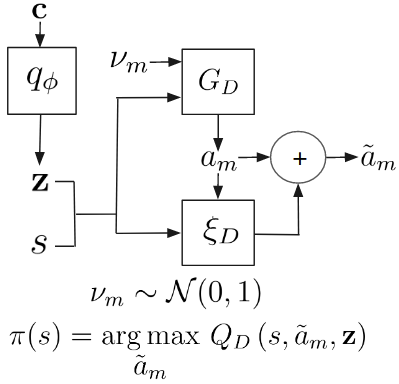
\includegraphics[width=0.6\textwidth]{chapter_2/fig/action-selection.png}
            \caption{Action selection. Given $s$, $G_D$ generates candidate actions $a_m$.
                $\xi_D$ generates small corrections for the actions $a_m$. The policy takes the corrected action $\tilde{a}_m$ with the highest value as estimated by $Q_D$.}
            \label{fig:action}
        \end{figure}
    \end{minipage}
\end{figure}

where $m$ is the triplet margin, $[\cdot]_{+}$ is the ReLU function and $d$ is a divergence measure. $q_\phi$ outputs the posterior over task identity, we thus choose $d$ to be the KL divergence.

Minimizing Eq. \ref{eq_triplet_task_i} accomplishes two goals. It encourages the task inference module $q_\phi$ to infer similar task identities when given either ${\bf c}_i$ or ${\bf c}_{j\rightarrow{i}}$ as input. It also encourages $q_\phi$ to infer different task identities for ${\bf c}_j$ and ${\bf c}_{j\rightarrow{i}}$. We emphasize that the task inference module can not learn to correlate \textit{only} the state-action pairs with the task identity since ${\bf c}_j$ and ${\bf c}_{j\rightarrow{i}}$ contain the same state-action pairs, but they correspond to different task identities. To minimize Eq. \ref{eq_triplet_task_i}, the module must model the correct conditional dependency $P(Z|S, A, R)$ when inferring the task identity.

Eq. \ref{eq_triplet_task_i} calculates the triplet loss when we use the learned reward function of task $i$ to relabel transitions from the remaining tasks. Following similar procedures for the remaining tasks lead to the loss:
\begin{equation}\label{eq_triplet_all_task}
    \mathcal{L}_{triplet} =  \frac{1}{K} \sum_{i=1}^{K} \mathcal{L}^i_{triplet}.
\end{equation}
The final loss to train the randomly initialized task inference module $q_\phi$, the distilled value functions $Q_D$, the distilled candidate action generator $G_D$, and the distilled perturbation generator $\xi_D$ is:
% from random initialization is:
\begin{equation}\label{eq_loss_final}
    % \mathcal{L} = \mathcal{L}_{triplet} + \mathcal{L}_{reg} + \mathcal{L}_{distill}
    \mathcal{L} = \mathcal{L}_{triplet} + \mathcal{L}_Q + \mathcal{L}_G + \mathcal{L}_\xi.
\end{equation}
Alg. \ref{algo_mtbrl} illustrates the pseudo-code for the second phase of the distillation procedure. Detailed pseudo-code of the two-phases distillation procedures can be found in \autoref{sec_detailed_distill}. Fig. \ref{fig:action} briefly describes action selection from the multi-task policy. \autoref{sec_action} provides detailed explanations. In theory, we can also use the relabelled transitions in Eq. \ref{eq_relabel} to train the single-task BCQ policy in the first phase, which we do not since we focus on task inference in this work.
